\documentclass[11pt, a4paper]{report}

% --- CÀI ĐẶT UNIVERSAL PREAMBLE ---
% Gói này rất quan trọng để hỗ trợ tiếng Việt
\usepackage{fontspec} % Cho phép chọn font
\usepackage{polyglossia}
\setdefaultlanguage{vietnamese}

% Cấu hình lề giấy
\usepackage[a4paper, top=2.5cm, bottom=2.5cm, left=2.5cm, right=2.5cm]{geometry}

% Chọn font Times New Roman cho chữ chính và JetBrains Mono cho code
\setmainfont{Times New Roman}
\setmonofont{JetBrains Mono}[Scale=0.9]

% Định nghĩa font riêng cho listings
\newfontfamily\listingsfont{JetBrains Mono}[Scale=0.9]

% Sửa lỗi hiển thị gạch đầu dòng (list bullets)
\usepackage{enumitem}
\setlist[itemize]{label=-}

% --- CÁC GÓI BỔ SUNG CHO BÁO CÁO NÀY ---
\usepackage{graphicx}     % Để chèn hình ảnh (biểu đồ)
\usepackage{booktabs}     % Cho bảng đẹp (bảng phân công)
\usepackage{listings}     % Để chèn code Java
\usepackage{xcolor}       % Để định nghĩa màu cho code
\usepackage{hyperref}     % Cho mục lục có thể nhấp vào (luôn để cuối cùng)

% Cấu hình màu sắc cho code listing
\definecolor{codegreen}{rgb}{0,0.6,0}
\definecolor{codegray}{rgb}{0.5,0.5,0.5}
\definecolor{codepurple}{rgb}{0.58,0,0.82}
\definecolor{backcolour}{rgb}{0.98,0.98,0.98}

% Cấu hình style cho code Java với XeLaTeX
\lstdefinestyle{mystyle}{
    backgroundcolor=\color{backcolour},
    commentstyle=\color{codegreen},
    keywordstyle=\color{magenta},
    numberstyle=\tiny\color{codegray},
    stringstyle=\color{codepurple},
    basicstyle=\listingsfont\footnotesize,
    breakatwhitespace=false,
    breaklines=true,
    captionpos=b,
    keepspaces=true,
    numbers=left,
    numbersep=5pt,
    showspaces=false,
    showstringspaces=false,
    showtabs=false,
    tabsize=2
}

% Cấu hình chung cho listings
\lstset{style=mystyle}

% --- BẮT ĐẦU TÀI LIỆU ---
\begin{document}

% --- TRANG BÌA ---
\begin{titlepage}
    \centering
    \sffamily

    % Cập nhật đường dẫn hình ảnh logo
    
\includegraphics[width=0.3\textwidth]{images/logo_sgu.png}
    \vspace{1cm}

    {\Large ỦY BAN NHÂN DÂN THÀNH PHỐ HỒ CHÍ MINH\par}
    {\LARGE \textbf{TRƯỜNG ĐẠI HỌC SÀI GÒN}\par}
    {\Large \textbf{KHOA CÔNG NGHỆ THÔNG TIN}\par}

    \vfill

    {\Huge \textbf{BÁO CÁO}}\par
    \vspace{0.5cm}
    {\Large HỌC PHẦN: KIỂM THỬ PHẦN MỀM (841408)}\par
    
    \vspace{1cm}
    {\Huge \textbf{CODE TECHNICAL REVIEW}}\par

    \vfill

    \begin{flushright}
    \large
    \begin{tabular}{ll}
        \textbf{Nhóm lớp:} & L01 \\
        \textbf{Giảng viên:} & ThS. Từ Lãng Phiêu \\
        \textbf{Nhóm thực hiện:} & 46 \\
    \end{tabular}
    \end{flushright}

    \vspace{0.5cm}

    \textbf{\large Danh sách thành viên:}\par
    \large Mai Trần Tuấn Kiệt – 3122560038\par

    \vfill

    {\large Thành phố Hồ Chí Minh, tháng 10 năm 2025\par}
\end{titlepage}

% --- MỤC LỤC ---
\tableofcontents
\newpage

% --- NẠP CÁC CHƯƠNG TỪ CÁC FILE RIÊNG ---
% --- CHƯƠNG 1: PHÂN CÔNG ---
\chapter{Phân công}

\section{Danh sách thành viên}
Nhóm 46 thực hiện bài tập này với một thành viên:
\begin{itemize}
    \item Mai Trần Tuấn Kiệt – 3122560038 (Leader)
\end{itemize}

\section{Bảng phân công công việc}
Do nhóm chỉ có một thành viên, thành viên duy nhất chịu trách nhiệm thực hiện toàn bộ các công đoạn của quy trình review code.
\begin{table}[htbp]
\centering
\caption{Bảng phân công công việc Nhóm 46}
\begin{tabular}{@{}lll@{}}
\toprule
\textbf{Họ và tên} & \textbf{MSSV} & \textbf{Nhiệm vụ} \\ \midrule
Mai Trần Tuấn Kiệt & 3122560038 & - Nghiên cứu checklist (66 mục) \\
 & & - Thực hiện review 22 file .java \\
 & & - Ghi nhận và tổng hợp lỗi vào file Excel \\
 & & - Phân tích, trực quan hóa dữ liệu (Python) \\
 & & - Viết báo cáo tổng kết \\ \bottomrule
\end{tabular}
\end{table}

\newpage
% --- CHƯƠNG 2: QUY TRÌNH ---
\chapter{Quy trình review code}

Quy trình review code của nhóm được thực hiện theo 3 bước chính: Chuẩn bị, Thực hiện và Tổng hợp.

\section{Chuẩn bị}
\begin{itemize}
    \item \textbf{Nghiên cứu Checklist:} Nghiên cứu và hiểu rõ 66 mục trong sheet \texttt{"Check list"} trong file \texttt{"Code Review Report Sample.xlsx"} được cung cấp. Các mục này được chia thành 6 loại (DEVIATION, OMISSION, DEFECT, AMBIGUITY, REDUNDANCE, và các mục con).
    \item \textbf{Chuẩn bị công cụ:} Sử dụng Microsoft Excel để ghi lại các phát hiện (file \texttt{nhom46\_code\_review.xlsx}) và Visual Studio Code để xem xét mã nguồn Java.
    \item \textbf{Mục tiêu:} Đối tượng review là 22 file mã nguồn \texttt{.java} của một dự án Web E-commerce.
\end{itemize}

\section{Thực hiện}
\begin{itemize}
    \item Tiến hành đọc và phân tích thủ công từng file \texttt{.java}.
    \item Đối với mỗi file, duyệt qua 66 mục của checklist để xác định các vi phạm.
    \item Khi phát hiện vi phạm, ghi lại thông tin vào sheet Excel tương ứng với file đó, bao gồm:
    \begin{itemize}
        \item \textbf{Check code:} Mã lỗi vi phạm (ví dụ: 15).
        \item \textbf{Check code Description:} Mô tả của mã lỗi.
        \item \textbf{Line:} Dòng code xảy ra vi phạm.
        \item \textbf{Comment:} Mô tả chi tiết về lỗi vi phạm.
        \item \textbf{Suggestion / Fix ?:} Đề xuất cách sửa lỗi.
    \end{itemize}
\end{itemize}

\section{Tổng hợp}
\begin{itemize}
    \item Sau khi hoàn tất review 22 file, toàn bộ dữ liệu từ các sheet Excel được tổng hợp lại.
    \item Sử dụng thư viện \texttt{pandas} và \texttt{matplotlib} của Python để phân tích và trực quan hóa dữ liệu tổng hợp.
    \item Các biểu đồ thống kê được tạo ra để cung cấp cái nhìn tổng quan về chất lượng mã nguồn (xem Chương 4).
    \item Viết báo cáo để trình bày lại toàn bộ quy trình, các phát hiện nghiêm trọng và kết quả thống kê.
\end{itemize}

\newpage
% --- CHƯƠNG 3: VẤN ĐỀ CHÍNH ---
\chapter{Các vấn đề và đề xuất}
Qua quá trình review, đã phát hiện tổng cộng \textbf{166 lỗi} trên 22 file. Dưới đây là các vấn đề nổi bật và nghiêm trọng nhất được phân loại theo mức độ ảnh hưởng.

\section{Lỗi Bảo mật Nghiêm trọng: SQL Injection (Hạng: Critical)}
\textbf{Vấn đề:} Đây là lỗi nghiêm trọng nhất, xuất hiện lặp lại ở hầu hết các class DAO (Data Access Object) như \texttt{BookDAO.java}, \texttt{UserDAO.java}, \texttt{OrderDAO.java}, và \texttt{SalesDAO.java}. Mã nguồn đang sử dụng phương thức cộng chuỗi (string concatenation) để xây dựng các câu lệnh SQL, cho phép kẻ tấn công chèn mã SQL độc hại và truy cập trái phép vào cơ sở dữ liệu.

\textbf{Ví dụ (từ \texttt{UserDAO.java}):}
\begin{lstlisting}[language=Java, caption={Lỗ hổng SQL Injection trong UserDAO.java (Line 25)}, firstnumber=25]
// Lỗi: Cộng chuỗi trực tiếp từ input của người dùng
String query = "SELECT * FROM user WHERE email = '" + email + "'";
// ...
ResultSet rs = st.executeQuery(query);
\end{lstlisting}

\textbf{Đề xuất:} Ngay lập tức thay thế \textbf{tất cả} các câu lệnh SQL cộng chuỗi bằng cách sử dụng \texttt{PreparedStatement}. \texttt{PreparedStatement} sẽ tự động xử lý và vô hiệu hóa các ký tự đặc biệt, ngăn chặn hoàn toàn các cuộc tấn công SQL Injection.

\textbf{Ví dụ sửa lỗi:}
\begin{lstlisting}[language=Java, caption={Sửa lỗi bằng PreparedStatement}]
// Sửa lỗi: Sử dụng PreparedStatement với tham số '?'
String query = "SELECT * FROM user WHERE email = ?";
PreparedStatement ps = connection.prepareStatement(query);
ps.setString(1, email);
ResultSet rs = ps.executeQuery();
\end{lstlisting}

\section{Lỗi Bảo mật Nghiêm trọng: Lộ thông tin nhạy cảm (Hạng: Critical)}
\textbf{Vấn đề:} File \texttt{ModelManager.java} (class quản lý kết nối CSDL) chứa thông tin đăng nhập (username và password) được \textbf{hardcode} (mã hóa cứng) trực tiếp trong mã nguồn. Điều này cực kỳ nguy hiểm vì bất kỳ ai có quyền truy cập vào mã nguồn đều có thể thấy và đánh cắp thông tin đăng nhập CSDL.

\textbf{Ví dụ (từ \texttt{ModelManager.java}):}
\begin{lstlisting}[language=Java, caption={Thông tin nhạy cảm bị hardcode (Line 8-10)}, firstnumber=8]
private static final String url = "jdbc:mysql://localhost:3306/bookstore";
private static final String dbuser = "root";
// Lỗi: Mật khẩu bị hardcode (dù đã bị comment)
// private static final String dbpass = "123456";
private static final String dbpass = "admin";
\end{lstlisting}

\textbf{Đề xuất:} Xóa ngay lập tức thông tin đăng nhập khỏi mã nguồn. Sử dụng các cơ chế an toàn hơn như biến môi trường (environment variables) hoặc file cấu hình (ví dụ: \texttt{.properties}, \texttt{.env}) để lưu trữ và tải thông tin này khi ứng dụng khởi chạy.

\section{Lỗi Bảo mật Cao: Mật mã yếu (Hạng: High)}
\textbf{Vấn đề:} Class \texttt{PasswordEncryptionService.java} chịu trách nhiệm mã hóa mật khẩu nhưng sử dụng các thuật toán và thông số đã lỗi thời, không còn an toàn:
\begin{itemize}
    \item \textbf{Thuật toán yếu:} Sử dụng \texttt{PBKDF2WithHmacSHA1}. Thuật toán SHA-1 đã bị xem là không an toàn, nên sử dụng SHA-256 hoặc SHA-512.
    \item \textbf{Số vòng lặp thấp:} Chỉ sử dụng 20000 vòng lặp. OWASP khuyến nghị số vòng lặp tối thiểu là 100,000 hoặc cao hơn.
    \item \textbf{Salt size nhỏ:} Kích thước salt chỉ là 8 bytes (64 bit), nên tăng lên ít nhất 16 bytes (128 bit) để chống lại các cuộc tấn công rainbow table.
\end{itemize}

\textbf{Đề xuất:} Nâng cấp ngay lập tức dịch vụ mã hóa mật khẩu:
\begin{itemize}
    \item Thay thế \texttt{PBKDF2WithHmacSHA1} bằng \texttt{PBKDF2WithHmacSHA512}.
    \item Tăng số vòng lặp (iteration count) lên ít nhất 100,000.
    \item Tăng kích thước salt (salt size) lên 16 hoặc 32 bytes.
\end{itemize}

\section{Xử lý ngoại lệ không đầy đủ (Hạng: Medium)}
\textbf{Vấn đề:} Lỗi này xuất hiện rất phổ biến (ví dụ: \texttt{Register.java}, \texttt{Statistics.java}). Khi một ngoại lệ (Exception) xảy ra, mã nguồn chỉ gọi \texttt{e.printStackTrace()}. Điều này không cung cấp thông báo lỗi thân thiện cho người dùng và không ghi lại lỗi một cách có hệ thống, khiến việc debug và bảo trì rất khó khăn.

\textbf{Đề xuất:}
\begin{itemize}
    \item Thay thế \texttt{e.printStackTrace()} bằng một framework ghi log (ví dụ: Log4j, SLF4J).
    \item Đối với các lỗi trong servlet, hãy chuyển hướng (forward) người dùng đến một trang lỗi (ví dụ: \texttt{error.jsp}) với thông báo lỗi rõ ràng.
\end{itemize}

\section{Nguy cơ NullPointerException (Hạng: Medium)}
\textbf{Vấn đề:} Nhiều phần của mã nguồn không kiểm tra giá trị \texttt{null} trước khi sử dụng, đặc biệt là khi lấy dữ liệu từ \texttt{request.getParameter()} (ví dụ: \texttt{Login.java}, \texttt{BookUpdate.java}) hoặc khi các phương thức DAO trả về \texttt{null}.

\textbf{Đề xuất:} Luôn luôn kiểm tra giá trị \texttt{null} đối với các biến có thể là \texttt{null} trước khi gọi phương thức trên chúng. Sử dụng \texttt{if (variable != null)} hoặc các kỹ thuật so sánh chuỗi an toàn như \texttt{"constant".equals(variable)}.

\section{Vi phạm quy ước và thiết kế (Hạng: Low)}
\textbf{Vấn đề:}
\begin{itemize}
    \item \textbf{Naming Convention:} Nhiều thuộc tính và phương thức sử dụng \texttt{snake\_case} (ví dụ: \texttt{book\_name}, \texttt{sum\_paid}) thay vì \texttt{camelCase} (ví dụ: \texttt{bookName}, \texttt{sumPaid}) theo chuẩn của Java.
    \item \textbf{Thiếu triển khai:} Toàn bộ class \texttt{Manager.java} chỉ chứa các phương thức rỗng, không có logic.
    \item \textbf{Thiếu Javadoc:} Hầu hết các class và phương thức đều thiếu Javadoc comment, gây khó khăn cho việc hiểu mục đích của mã.
\end{itemize}

\textbf{Đề xuất:} Thực hiện một đợt refactor toàn diện để đổi tên các biến/phương thức theo chuẩn \texttt{camelCase} và bổ sung Javadoc cho các class quan trọng.

\newpage
% --- CHƯƠNG 4: THỐNG KÊ ---
\chapter{Trực quan hóa dữ liệu thống kê}
Để có cái nhìn tổng quan về kết quả review, dữ liệu lỗi đã được tổng hợp và trực quan hóa bằng Python.

\begin{figure}[htbp]
  \centering
  % Cập nhật đường dẫn hình ảnh
  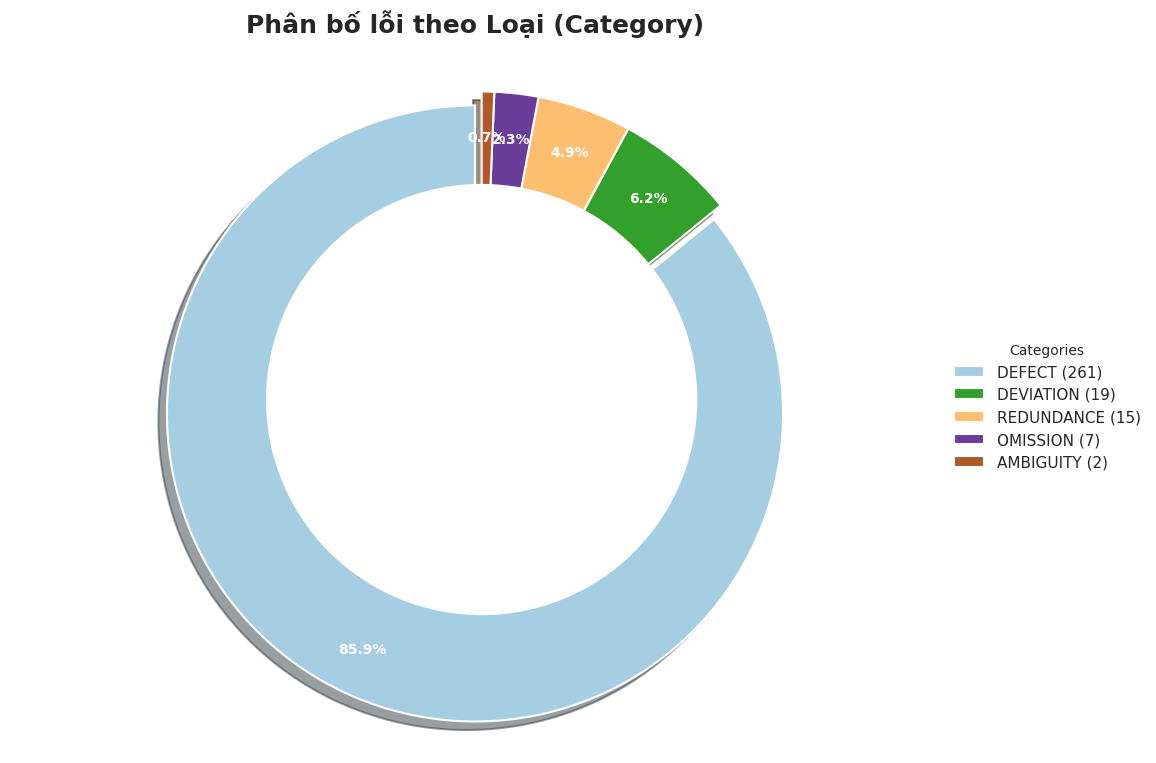
\includegraphics[width=0.9\textwidth]{images/bieu_do_pie_category.png}
  \caption{Tỷ lệ phân bố lỗi theo 5 loại chính (Category). Đa số lỗi thuộc nhóm DEFECT (khiếm khuyết trong logic).}
  \label{fig:pie_chart}
\end{figure}

\begin{figure}[htbp]
  \centering
  % Cập nhật đường dẫn hình ảnh
  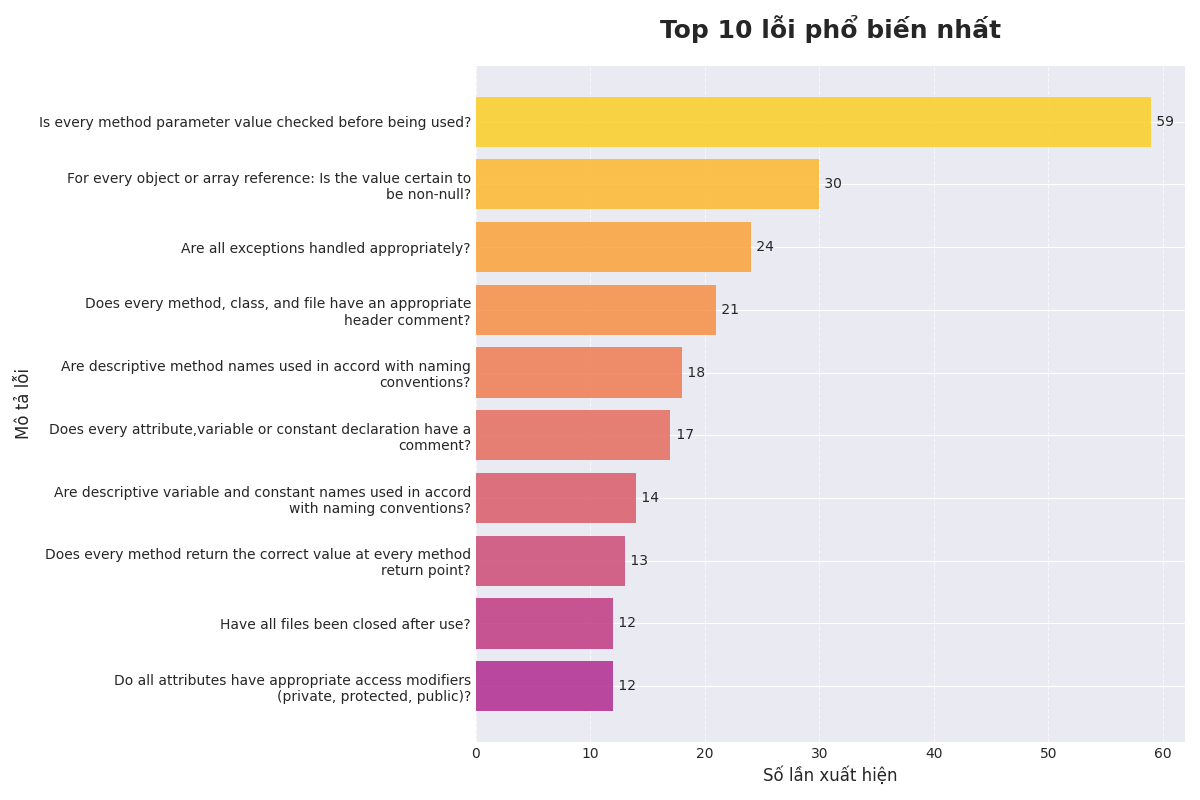
\includegraphics[width=1\textwidth]{images/bieu_do_top_10_loi.png}
  \caption{Top 10 lỗi phổ biến nhất. Lỗi "thiếu kiểm tra tham số" (Mã 15) là phổ biến nhất và cũng là nguyên nhân chính gây ra lỗi SQL Injection.}
  \label{fig:top10_chart}
\end{figure}

\begin{figure}[htbp]
  \centering
  % Cập nhật đường dẫn hình ảnh
  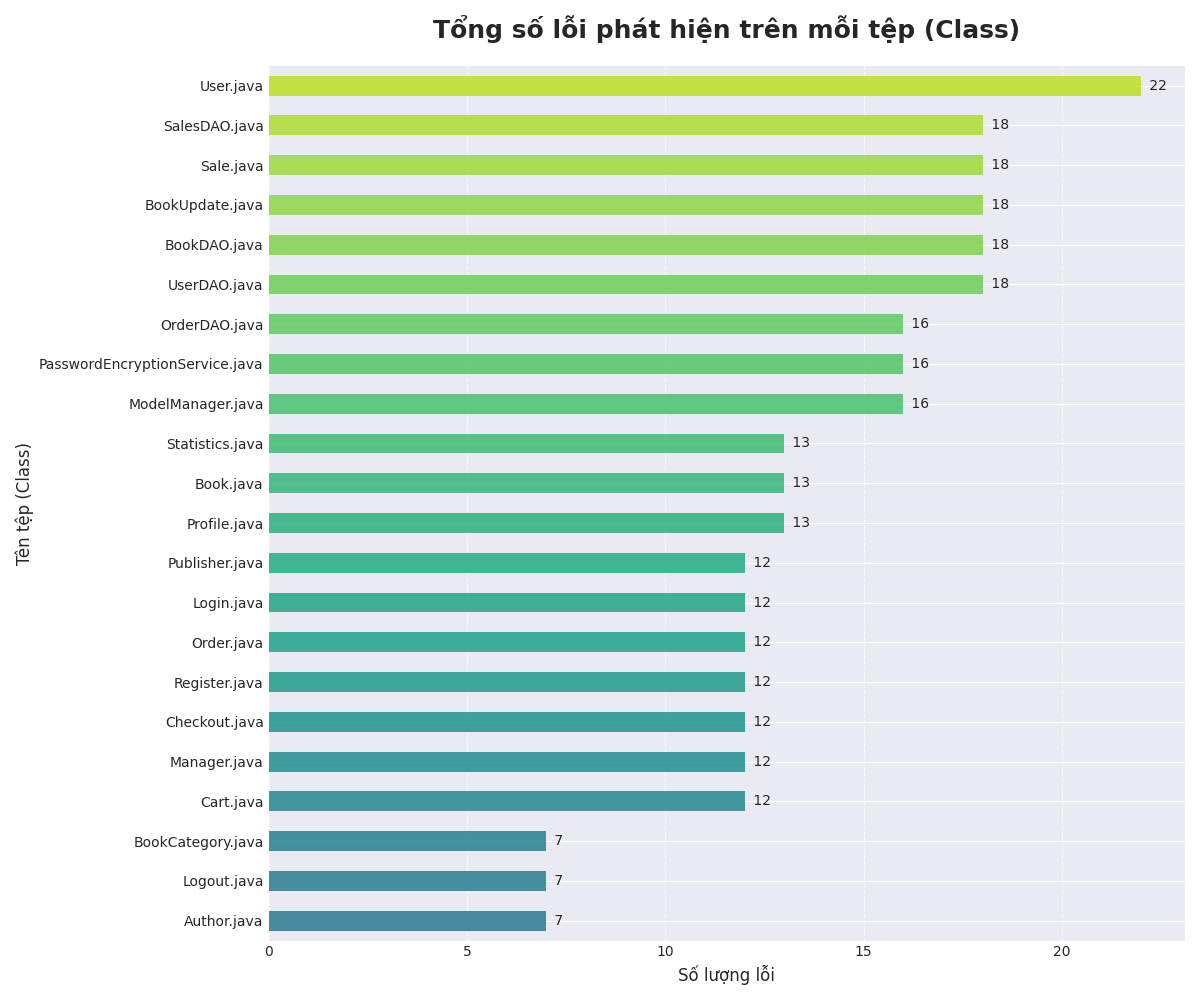
\includegraphics[width=1\textwidth]{images/bieu_do_loi_moi_tep.png}
  \caption{Phân bố số lượng lỗi trên từng tệp. \texttt{BookDAO.java} và \texttt{BookUpdate.java} là hai file có nhiều vấn đề nhất.}
  \label{fig:files_chart}
\end{figure}

\begin{figure}[htbp]
  \centering
  % Cập nhật đường dẫn hình ảnh
  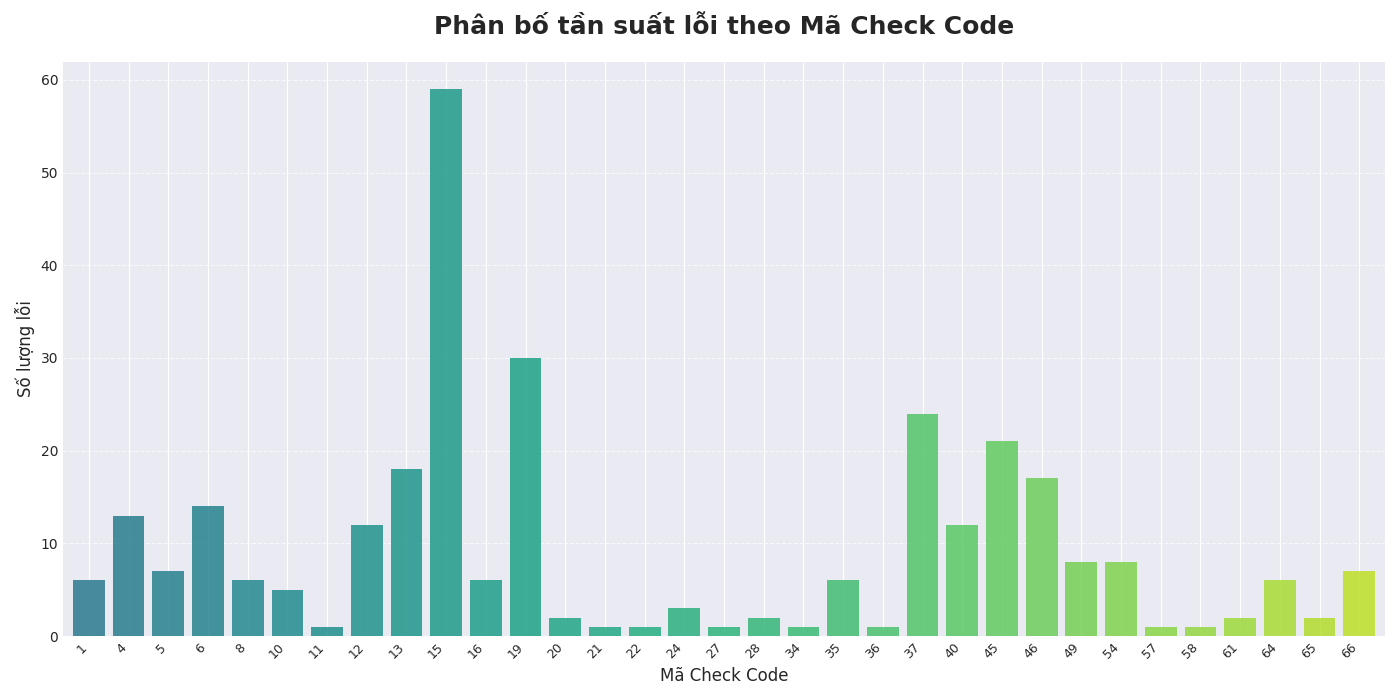
\includegraphics[width=1\textwidth]{images/bieu_do_phan_bo_loi.png}
  \caption{Tần suất xuất hiện của từng mã lỗi (Check code).}
  \label{fig:checkcode_chart}
\end{figure}

\newpage
% --- CHƯƠNG 5: KẾT LUẬN ---
\chapter{Kết luận}

Quá trình review code thủ công \textbf{22 file} mã nguồn Java đã phát hiện tổng cộng \textbf{304 lỗi} vi phạm checklist.
Số loại lỗi (theo Check code) riêng biệt: \textbf{33 lỗi}.
Phân tích thống kê cho thấy các vấn đề nghiêm trọng nhất không chỉ tồn tại mà còn lặp lại một cách có hệ thống, tập trung vào các nhóm lỗi:
\begin{enumerate}
    \item \textbf{DEFECT (65.7\%):} Chiếm đa số, bao gồm các lỗi nghiêm trọng nhất như SQL Injection, mật khẩu hardcode, và mật mã yếu.
    \item \textbf{DEVIATION (22.9\%):} Chủ yếu là vi phạm quy ước đặt tên (naming convention).
\end{enumerate}

Các file DAO (\texttt{BookDAO.java}, \texttt{UserDAO.java}, \texttt{SalesDAO.java}) và các Servlet (\texttt{BookUpdate.java}) là những nơi tập trung nhiều lỗi nhất và cũng là những nơi cần được ưu tiên sửa chữa.

\textbf{Đề xuất:} Dự án ở trạng thái \textbf{không an toàn} để triển khai (deploy) lên môi trường production.
Nhóm phát triển cần:
\begin{itemize}
    \item \textbf{Ưu tiên 1 (Critical):} Sửa toàn bộ các lỗ hổng SQL Injection bằng \texttt{PreparedStatement} và gỡ bỏ toàn bộ thông tin nhạy cảm (credentials) ra khỏi mã nguồn.
    \item \textbf{Ưu tiên 2 (High):} Nâng cấp dịch vụ mã hóa mật khẩu.
    \item \textbf{Ưu tiên 3 (Medium/Low):} Thực hiện refactor để xử lý NullPointerException, đóng tài nguyên (resource leaks) và chuẩn hóa lại quy ước đặt tên.
\end{itemize}

\end{document}